\section{Porównanie implementacji w Matlabie oraz w C++}

Istotną sprawą jest sprawdzenie, czy występują znaczące różnice między implementacją w Matlabie oraz w C++. W celu porównania sprawdzono rozbieżności pomiędzy implementacjami (wizualnie) oraz czas obliczeń.

\subsection{Rozbieżności między implementacjami}

W celu porównania rezultatów uzyskanych w Matlabie oraz w C++ dokonano próby odszumienia sygnału oznaczonego numerem 100 (pierwsze 100000 próbek) pochodzącego z Physionet MIT-BIH arrythymia database\cite{mitbih} obydwoma programami. Parametry algorytmu w obu przypadkach są takie same (domyślne). Następnie zestawiono wyniki na wspólnym wykresie.

\begin{figure}[!htb]
	\begin{center}
		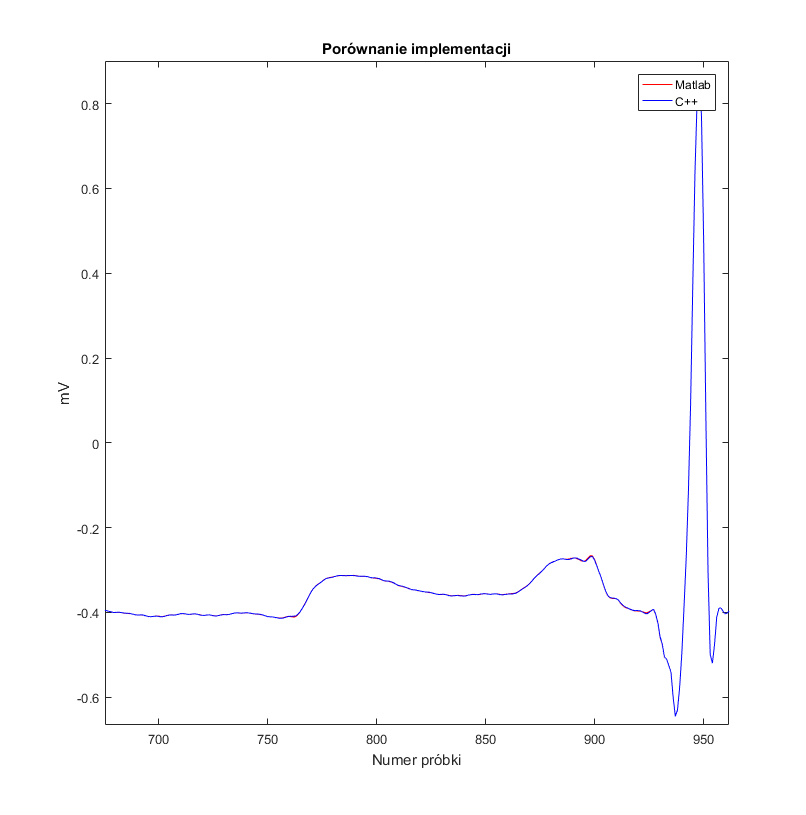
\includegraphics[width=15cm,clip]
		{img/porownanie.png}
	\end{center}
	\caption{Porównanie obydwu implementacji. Wykres został przybliżony na jeden pseudookres, ze względu na brak czytelności wykresu. }
	\label{rys:porownanie}
\end{figure}

Rysunek \ref{rys:porownanie} dowodzi, że implementacja w C++ i w Matlabie dają podobne rezultaty. Nieznaczne różnice mogą wynikać z różnic pomiędzy precyzjami typów \texttt{double} w obu językach.

\subsection{Czasowe porównanie implementacji}

Obydwie implementacje dają podobne rezultaty. Można zatem porównać czas wykonywania obydwu programów. Programy zostały uruchomione na komputerze z procesorem Intel i7 4790.
\begin{table}[!htb]
	\centering
	\caption{Tabela porównująca czasy wykonania programu.}
	\begin{tabular}{|c|l|l|}
		\hline
		Język & Czas [$\mathrm{s}$] \\
		\hline
		Matlab & 96,958 \\
		\hline
		C++ & 22,937 \\
		\hline
	\end{tabular}
	\label{tab:tabela2}
\end{table}

Niekwestionowanym zwycięzcą jest C++. Warto jednak zauważyć, że bez flagi \texttt{-Ofast} program w C++ wykonuje się znacznie dłużej (dla takiego samego zestawu danych - kilkanaście minut).

Czas wykonywania programu może wydawać się bardzo długi, jednak jest on związany z dużą złożonością obliczeniową. Wykonywane są 3 zagnieżdżone w sobie pętle. Dla parametrów domyślnych instrukcje z wewnętrznej pętli programu wykonują się około $(n-2P-1)\cdot(2M+1)\cdot(2P+1)$ razy, co dla domyślnych parametrów i serii 100 tysięcy próbek daje około 8 miliardów iteracji.